\documentclass[12pt,a4paper]{article}

\input{../preamble_files/packages}
\input{../preamble_files/figures}
\input{../preamble_files/references}
\input{../preamble_files/shortcuts}
\input{../preamble_files/listings}

\pagestyle{fancy}
\lhead{Richard Whitehill}
\chead{MATH 551 -- HW 1}
\rhead{02/10/22}
\cfoot{\thepage~of~\pageref{LastPage}}

\newcommand{\prob}[2]{\textbf{#1)} #2}

\setlength{\parskip}{\baselineskip}
\setlength{\parindent}{0pt}

\begin{document}

\prob{1}{Prove that the following equations have at least one solution in the given intervals.}

(a) $x - (\ln{x})^3 = 0,\quad [5,7]$

$\rightarrow$ Notice that $5 - (\ln{5})^3 \approx 0.831 > 0$ and $7 - (\ln{7})^3 \approx -3.68 < 0$. Hence by the Intermediate Value Theorem (IVT), we are guranteed that at least one solution to the above equation exists on the compact interval between 5 and 7 since the function $f(x) = x - (\ln{x})^3$ is continuous on $\reals$.

(b) $5x\cos(\pi x) - 2x^2 + 3 = 0,\quad [0,2]$

$\rightarrow$ Notice that $5(0)\cos(\pi (0)) - 2(0)^2 + 3 = 3 > 0$ and $5(1)\cos(\pi) - 2(1)^2 + 3 = -5 - 2 + 3 = -4 < 0$. Thus, we a solution to the above equation exists in the interval $[0,2]$ by the IVT, given that $f(x) = 5x\cos(\pi x) - 2x^2 + 3$ is continuous on $\reals$. In fact, we are guranteed a solution exists on $[0,1]$ and $[0,2]$, observing that $5(2)\cos(2\pi) - 2(2)^2 + 3 = 10 - 8 + 3 = 5 > 0$.  

\prob{2}{Verify that the function $|| \cdot ||_1$ defined on $\reals^n$ by
\begin{align*}
||\vec{x}||_1 = \sum_{i=1}^{n} |x_i|
\end{align*}
is a norm on $\reals^n$.}

$\rightarrow$ We show that $||\cdot||_1$ is a norm by proving that it satisfies the following properties. Let $\vec{x} = (x_1,\hdots, x_n)^{T} \in \reals^n$.

i) Observe that $||\vec{x}||_1 \geq 0$ since for each $i$ we have $|x_i| \geq 0$, meaning the sum $\sum_{i=1}^{n} |x_i| \geq 0$. Furthermore, notice that if $\vec{x} = 0$, then $\sum_{i=1}^{n} |0| = 0$, and if $\sum_{i=1}^{n} |x_i| = 0$, then for each $i$ we must have $|x_i| = 0$, implying that $\vec{x} = 0$.

ii) Let $\alpha \in \reals$. Observe that $||\alpha\vec{x}||_1 = \sum_{i=1}^{n} |\alpha x_i| = \sum_{i=1}^{n} |\alpha||x_i| = |\alpha|\sum_{i=1}^{n} |x_i|= |\alpha|||\vec{x}||_1$.

iii) It can be shown that for any two real numbers $x,y$ that the following inequality holds: $|x+y| \leq |x| + |y|$. Hence we have $||\vec{x} + \vec{y}||_1 = \sum_{i=1}^{n} |x_i + y_i| \leq \sum_{i=1}^{n} (|x_i| + |y_i|) = \sum_{i=1}^{n} |x_i| + \sum_{i=1}^{n} |y_i| = ||\vec{x}||_1 + ||\vec{y}||_1$.

Since 

\prob{3}{Find $l_1,~l_2,~\text{ and }l_{\infty}$ norms of the following vectors or matrices.}

(a) $x = (2,1,-3,4)^{T}$
\begin{align*}
||x||_1 &= |2| + |1| + |-3| + |4| = 2 + 1 + 3 + 4 = 10 \\
||x||_2 &= \sqrt{(2)^2 + (1)^2 + (-3)^2 + (4)^2} = \sqrt{4 + 1 + 9 + 16} = \sqrt{30} \\
||x||_{\infty} &= \max\{|2|,|1|,|-3|,|4|\} = 4
\end{align*}

(b) $x = (\sin{k},\cos{k},2^{k})^{T}$
\begin{align*}
||x||_1 &= |\sin{k}| + |\cos{k}| + 2^{k} \\
||x||_2 &= \sqrt{\sin^{2}{k} + \cos^{2}{k} + (2^{k})^2} = \sqrt{1 + 4^{k}} \\
||x||_{\infty} &= \max\{|\sin{k}|,|\cos{k}|,2^k\} = 2^{k}
\end{align*}

(c) 
\[
\begin{bmatrix}
10 & 15 \\
0  & 1
\end{bmatrix}
\]
\begin{align*}
||A||_1 &= \max\{|10|+|0|,|15|+|1|\} = 16 \\
||A||_{\infty} &= \max\{|10|+|15|,|0|+|1|\} = 25 \\
||A||_{2} &= \sqrt{\rho(A^{T}A)} = \sqrt{\max\{163 \pm 3\sqrt{2941}\}} \\
&= \sqrt{163 + 3\sqrt{2941}} \approx 18.047
\end{align*}\\

(d) 
\[
\begin{bmatrix}
2 & -1 & 0 \\
-1 & 2 & -1 \\
0 & -1 & 2
\end{bmatrix}
\]
\begin{align*}
||A||_1 &= \max\{|2|+|-1|+|0|,|-1|+|2|+|-1|,|0|+|-1|+|2|\} = 4 \\
||A||_{\infty} &= 4 \text{ (since the matrix is symmetric about the diagonal)} \\
||A||_{2} &= \sqrt{\max\{4,6 \pm 4\sqrt{2}\}} = \sqrt{6 + 4\sqrt{2}} \approx{11.657}
\end{align*}

Note: I used the \textit{sympy} package in python to solve for the eigenvalues of $A^{T}A$.

\prob{4}{Taylor expand the following function.}

(a) $e^x$ around $x = 0$
\begin{align*}
e^{x} = 1 + x + \frac{x^{2}}{2} + \frac{x^{3}}{6} + \frac{x^{4}}{24} + \frac{x^{5}}{120} + \frac{x^{6}}{720} + \frac{x^{7}}{5040} + O\left(x^{8}\right)
\end{align*}

(b) $\log(x+1)$ around $x = 0$
\begin{align*}
\log(x+1) = x - \frac{x^{2}}{2} + \frac{x^{3}}{3} - \frac{x^{4}}{4} + \frac{x^{5}}{5} - \frac{x^{6}}{6} + \frac{x^{7}}{7} + O\left(x^{8}\right)
\end{align*}

\inputpython{prob4.py}

\prob{5}{Plot the function $e^x$ on $[0,1]$ in a black solid line. On the same graph, plot the function $1+x+\frac{x^2}{2!}$ in blue circle.}

\bef
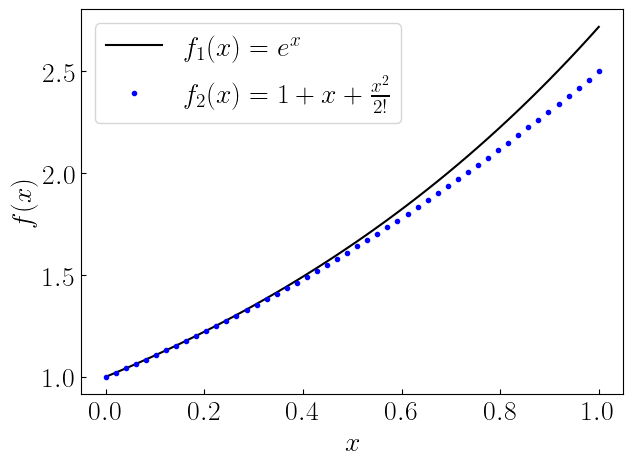
\includegraphics[scale=0.75]{prob5fig.png}
\eef

\inputpython{prob5.py}



\end{document}
